\documentclass[12pt]{article}
\usepackage[sc]{mathpazo}
\usepackage{commands}
\hypersetup{colorlinks = true}
\let\oldphi\phi 
\let\phi\varphi 
\let\varphi\oldphi



\begin{document}

\heading{The Complex Analysis and Applications}

The content of this lecture note will be mostly based on the course MATH 305 (Applied Complex Analysis) at UBC during Winter2, 2023 term. However, I have expanded the content and examples using the following text books as well:



\begin{itemize}
\item Fundamentals of Complex Analysis for Mathematics, Science and Engineering,(Third Edition) by E. Saff, A. Snider.
\item Visual Complex Functions: An Introduction with Phase Portraits by Elias Wegert
\end{itemize}



\newpage
\section{Basics}
Partial differential equations relate the partial derivatives of a function to each other. For example $f$ can be a function of spacial coordinates (like $x,y,z$ in the case of Cartesian coordinates), dynamical variable (like time), or any other kind of variables (like the space of genotypes g). For example suppose that $ \Phi(x,y) $ represents the electric potential of a point charge. Such function should satisfy the Laplace equation:

\[	 \partial_{xx} \Phi + \partial_{yy} \Phi = 0.	\]
Note that the symbols $ \partial_{xx} $ and $ \partial_{yy} $ are short symbols for $ \frac{\partial^2}{\partial x^2} $ and $ \frac{\partial^2}{\partial y^2} $ respectively.

\begin{defbox}{Order of PDE}
	The order of a PDE is the highest derivative that occurs in the equation. 
\end{defbox}

Based on the definition above, the Laplace equation is a second order partial differential equation. 

\subsection{Classification of The Second Order PDEs }

There are three categories of the second order PDEs that every other type of a second order PDE can be converted to one of these kinds. The most general type of a second order PDE can be written as:

\begin{equation}
	A \partial_{xx} u + B \partial_{xy} u + C \partial_{yy} u + D \partial_{x} u + E \partial_{y} u + F u = k
	\label{equ:GeneralSecondOrderPDE}
\end{equation}

In which the coefficients are all a function of $x,y$ (but not $ u $ in which case the PDE will be nonlinearx). Equation \ref{equ:GeneralSecondOrderPDE} can be summarized in a more compact form using the derivative operator $ \operatorname{L} $: 

\[	 \operatorname{L} u = 0,	\]

in which:

\[  \operatorname{L} = A \partial_{xx} + B \partial_{xy} + C \partial_{yy} + D \partial_{x} + E \partial_{y} + F \].

Because of the similarities of the equation \ref{equ:GeneralSecondOrderPDE} with the generic quadratic equation describing the conic sections, we call each class of second order PDEs with its corresponding conic section. The generic equation describing the conic sections is:

\begin{equation}
	A x^2 + B x y + C y^2 + D x + E y + K = 0.
	\label{equ:ConicSections}
\end{equation}


All of the conic sections (ellipse, parabola, hyperbola) can be described with the equation \ref{equ:ConicSections} which is determined with the discriminant $ \Delta = B^2 - 4 A C $. for $ \Delta=0 $, $ \Delta > 0 $, and $ \Delta < 0 $ the conic section will be \textbf{parabolic}, \textbf{hyperbolic}, and \textbf{elliptic} respectively. Table \ref{tab:PDE-types} summarizes special categories of the linear second order PDEs that frequently occur in physical applications. \newline


\begin{table}[]
	\centering
	\resizebox{\textwidth}{!}{%
		\begin{tabular}{|c|c|c|c|c|}
			\hline
			PDE                     & Analogous conic sec. & $\Delta$     & Class      & Application               \\ \hline
			$ u_t = u_{xx}$         & $T = x^2$           & 0            & parabolioc & Diffusion - Heat Equation \\ \hline
			$ u_{tt} = u_{xx} $     & $T^2 = x^2$         & $\Delta > 0$ & Hyperbolic & Wave Equation             \\ \hline
			$ u_{xx} + u_{yy} = 0 $ & $x^2 + y^2 = 0$ & \multirow{2}{*}{$\Delta < 0$} & \multirow{2}{*}{Elliptic} & Laplace \\ \cline{1-2} \cline{5-5} 
			$ u_{xx} + u_{yy} = c $ & $x^2 + y^2 = k$     &              &            & Poisson                   \\ \hline
		\end{tabular}%
	}
	\caption{A summary of the three class of second order linear PDE.}
	\label{tab:PDE-types}
\end{table}


\subsection{Intuitive Derivation of the Second Order PDEs}
The three classes of the second order linear PDEs in table \ref{tab:PDE-types} can be derived intuitively using the continuity law (conservation law) and the constitutive law that is determined by the nature of the problem which is the subject of the following sections. 
 
\subsubsection{Continuity Equation or Conservation Laws}
The most important part of deriving the PDE equations is the continuity law or conservation law. This fact is imposed because of our common sense about nature. Suppose that we want to study the concentration of of a red ink in a infinitesimal cube. The continuity equation, in simple terms, state that the change of the concentration of the ink inside the infinitesimal cube is equal to the ink that has entered the cube from outside from its boundaries (we are assuming no source or sink of ink inside the cube). For instance, consider the infinitesimal box in figure \ref{fig:infbox}. The change of the concentration of the ink inside the cube is $\frac{\partial c}{\partial t}$. Because we know that there are no sources or sinks of ink inside the cube, then the change in the concentration is equal to the amount that comes in and goes out from the boundaries of the box. To put this in numbers, we introduce the important vector quantity \emph{flux} $ \Phi $. Flux is the amount of particles flow per unit area per unit time (see figure \ref{fig_fluxCrossSection}).


\begin{figure}[h!]
	\centering
	\tikzset{every picture/.style={line width=0.75pt}} %set default line width to 0.75pt        
	
	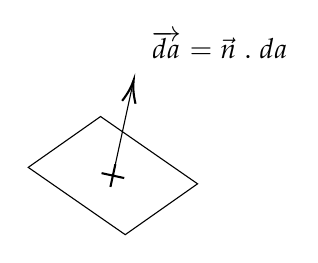
\begin{tikzpicture}[x=0.75pt,y=0.75pt,yscale=-1,xscale=1]
		%uncomment if require: \path (0,300); %set diagram left start at 0, and has height of 300
		
		%Flowchart: Data [id:dp7886171984971329] 
		\draw   (233.06,82.54) -- (279.79,114.96) -- (244.94,139.46) -- (198.21,107.04) -- cycle ;
		%Straight Lines [id:da19634912279776984] 
		\draw    (239,111) -- (248.58,66.95) ;
		\draw [shift={(249,65)}, rotate = 102.26] [color={rgb, 255:red, 0; green, 0; blue, 0 }  ][line width=0.75]    (10.93,-3.29) .. controls (6.95,-1.4) and (3.31,-0.3) .. (0,0) .. controls (3.31,0.3) and (6.95,1.4) .. (10.93,3.29)   ;
		\draw [shift={(239,111)}, rotate = 282.26] [color={rgb, 255:red, 0; green, 0; blue, 0 }  ][line width=0.75]    (-5.59,0) -- (5.59,0)(0,5.59) -- (0,-5.59)   ;
		
		% Text Node
		\draw (256,40) node [anchor=north west][inner sep=0.75pt]   [align=left] {$\displaystyle \overrightarrow{da} =\vec{n} \ .\ da$};
	\end{tikzpicture}
	\caption{The dot product $\protect\overrightarrow{\Phi}.\protect\overrightarrow{da}$ is the amount of particles passing through the infinitesimal cross section in unit time.}
	\label{fig_fluxCrossSection}
\end{figure}


\begin{figure}[h!]
	\centering
	\tikzset{every picture/.style={line width=0.75pt}} %set default line width to 0.75pt        
	
	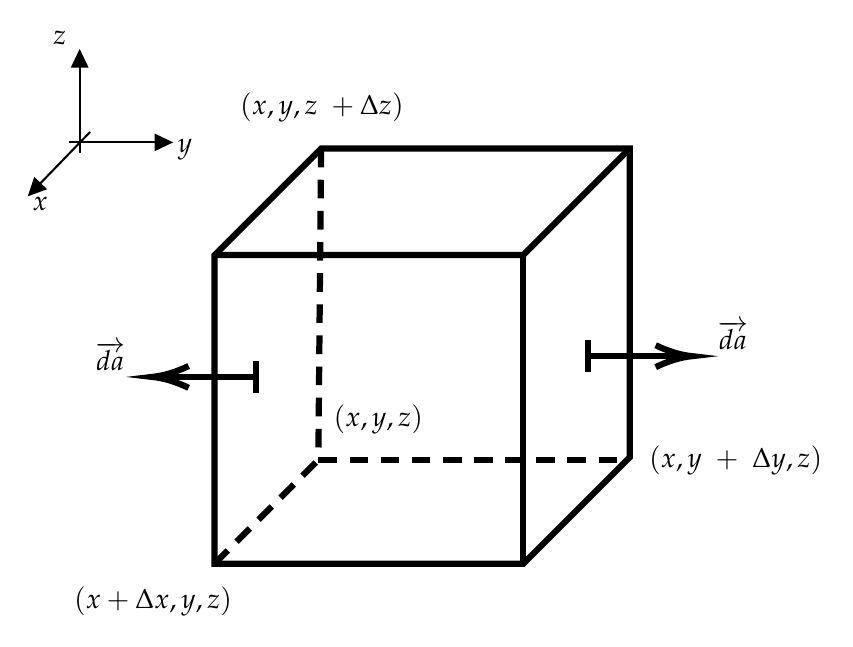
\begin{tikzpicture}[x=0.75pt,y=0.75pt,yscale=-1,xscale=1]
		%uncomment if require: \path (0,300); %set diagram left start at 0, and has height of 300
		
		%Shape: Cube [id:dp6052690098400888] 
		\draw  [line width=2.25]  (200,101.31) -- (251.31,50) -- (400,50) -- (400,198.69) -- (348.69,250) -- (200,250) -- cycle ; \draw  [line width=2.25]  (400,50) -- (348.69,101.31) -- (200,101.31) ; \draw  [line width=2.25]  (348.69,101.31) -- (348.69,250) ;
		%Straight Lines [id:da6838346844891714] 
		\draw [line width=2.25]  [dash pattern={on 6.75pt off 4.5pt}]  (250,200) -- (400,200) ;
		%Straight Lines [id:da4358863669422177] 
		\draw [line width=2.25]  [dash pattern={on 6.75pt off 4.5pt}]  (251.31,50) -- (250,200) ;
		%Straight Lines [id:da8699451449684632] 
		\draw [line width=2.25]  [dash pattern={on 6.75pt off 4.5pt}]  (200,250) -- (250,200) ;
		%Straight Lines [id:da6153923820857115] 
		\draw [line width=2.25]    (220,160) -- (174,160) ;
		\draw [shift={(170,160)}, rotate = 360] [color={rgb, 255:red, 0; green, 0; blue, 0 }  ][line width=2.25]    (17.49,-5.26) .. controls (11.12,-2.23) and (5.29,-0.48) .. (0,0) .. controls (5.29,0.48) and (11.12,2.23) .. (17.49,5.26)   ;
		\draw [shift={(220,160)}, rotate = 360] [color={rgb, 255:red, 0; green, 0; blue, 0 }  ][line width=2.25]    (0,7.83) -- (0,-7.83)   ;
		%Straight Lines [id:da3502060568264709] 
		\draw [line width=2.25]    (380,150) -- (426,150) ;
		\draw [shift={(430,150)}, rotate = 180] [color={rgb, 255:red, 0; green, 0; blue, 0 }  ][line width=2.25]    (17.49,-5.26) .. controls (11.12,-2.23) and (5.29,-0.48) .. (0,0) .. controls (5.29,0.48) and (11.12,2.23) .. (17.49,5.26)   ;
		\draw [shift={(380,150)}, rotate = 180] [color={rgb, 255:red, 0; green, 0; blue, 0 }  ][line width=2.25]    (0,7.83) -- (0,-7.83)   ;
		%Straight Lines [id:da8422422028495438] 
		\draw [line width=0.75]    (140,42) -- (112.09,70.84) ;
		\draw [shift={(110,73)}, rotate = 314.06] [fill={rgb, 255:red, 0; green, 0; blue, 0 }  ][line width=0.08]  [draw opacity=0] (8.93,-4.29) -- (0,0) -- (8.93,4.29) -- cycle    ;
		%Straight Lines [id:da7449366310627421] 
		\draw [line width=0.75]    (135,52) -- (135,5) ;
		\draw [shift={(135,2)}, rotate = 90] [fill={rgb, 255:red, 0; green, 0; blue, 0 }  ][line width=0.08]  [draw opacity=0] (8.93,-4.29) -- (0,0) -- (8.93,4.29) -- cycle    ;
		%Straight Lines [id:da9487980467676893] 
		\draw [line width=0.75]    (130,47) -- (177,47) ;
		\draw [shift={(180,47)}, rotate = 180] [fill={rgb, 255:red, 0; green, 0; blue, 0 }  ][line width=0.08]  [draw opacity=0] (8.93,-4.29) -- (0,0) -- (8.93,4.29) -- cycle    ;
		
		% Text Node
		\draw (256,172) node [anchor=north west][inner sep=0.75pt]   [align=left] {$\displaystyle ( x,y,z)$};
		% Text Node
		\draw (131,260) node [anchor=north west][inner sep=0.75pt]   [align=left] {$\displaystyle ( x+\Delta x,y,z)$};
		% Text Node
		\draw (408,192) node [anchor=north west][inner sep=0.75pt]   [align=left] {$\displaystyle ( x,y\ +\ \Delta y,z)$};
		% Text Node
		\draw (211,22) node [anchor=north west][inner sep=0.75pt]   [align=left] {$\displaystyle ( x,y,z\ +\Delta z)$};
		% Text Node
		\draw (111,72) node [anchor=north west][inner sep=0.75pt]   [align=left] {$\displaystyle x$};
		% Text Node
		\draw (181,44) node [anchor=north west][inner sep=0.75pt]   [align=left] {$\displaystyle y$};
		% Text Node
		\draw (121,-8) node [anchor=north west][inner sep=0.75pt]   [align=left] {$\displaystyle z$};
		% Text Node
		\draw (141,142) node [anchor=north west][inner sep=0.75pt]   [align=left] {$\displaystyle \overrightarrow{da}$};
		% Text Node
		\draw (441,132) node [anchor=north west][inner sep=0.75pt]   [align=left] {$\displaystyle \overrightarrow{da}$};
		
		
	\end{tikzpicture}
	\caption{The infinitesimal cube for deriving the continuity equation}
	\label{fig:infbox}
\end{figure}



\newpage

Let's get back to the infinitesimal cube in figure \ref{fig:infbox} and derive the continuity equation. We can start we tracking the net change in the number of particles inside the cube due to the flux in x direction:

\begin{align*}
	-\frac{dN_x}{dt} &= \Phi_x(x,y,z) . (-dz dy) + \Phi_x(x +dx, y,z) . (dzdy) \\
	 				&= (\Phi_x(x+dx,y,z)-\Phi_x(x,y,z))dydz 
\end{align*}

Note that the negative sign in the LHS of the equation above is simply to match the meaning of the two sides of the equations. For instance, if the RHS of the equation above is positive, it means that the net change of the number of particles in the box in negative (meaning that particles are leaving the box) which is equivalent to $ -\frac{dN}{dt} $. Similarly in the y and z direction:

\begin{align*}
	-\frac{dN_y}{dt} &= (\Phi_y(x,y+dy,z)-\Phi_y(x,y,z)) dx dz \\
	-\frac{dN_z}{dt} &= (\Phi_z(x,y,z+dz) - \Phi_z(x,y,z)) dx dy
\end{align*}

So the net change in the number of particle in the box per $dt$ will be:

\begin{align*}
	-\frac{dN}{dt} &= - (\frac{dN_x}{dt} + \frac{dN_y}{dt} + \frac{dN_z}{dt}) \\
	&= (\Phi_x(x+dx,y,z)-\Phi_x(x,y,z))dydz + \\
	&\, (\Phi_y(x,y+dy,z)-\Phi_y(x,y,z)) dx dz + \\
	&\, (\Phi_z(x,y,z+dz) - \Phi_z(x,y,z)) dx dy
\end{align*}


By dividing the both sides of the above equation by the volume of the cube $ dV = dx dy dz $ we can write:

\begin{equation*}
	\frac{dc}{dt} = - (\partial_{x}\Phi_x + \partial_{y}\Phi_y + \partial_{z}\Phi_z) = -\mathbf{\nabla} . \Phi
\end{equation*}

In which $c = N/V$ is the concentration, $ \nabla $ is the divergence operator, and $ \Phi $ is the flux. 

\begin{defbox}{Continuity Equation}
	The following important relation is known as the continuity equation(or conservation law):
	
	\begin{equation}
			\frac{dc}{dt} + \mathbf{\nabla} . \Phi = 0
	\end{equation}

	in which $\Phi$ is the flux, $c$ is the concentration, and $ \nabla $ is the divergence operator.
\end{defbox}


\subsubsection{Conservation Law for Momentum}
will be used to derive the wave equation


\subsection{Constitutive Laws: Advection, Diffusion and Wave Equation}

Having the continuity equation in hand makes the derivation PDEs very straight forward. We only need to insert the constitutive laws (which are enforced by the nature of the problem) in the continuity equations derived in the section above.


\begin{itemize}
	\item Fick's Law $\rightarrow$ Constitutive law for diffusion 
	\item Hook's law $\rightarrow$ Constitutive law for the wave equation
\end{itemize}






\end{document}